\documentclass[tikz,crop]{standalone}
%%% Tikz Libraries %%%
\usetikzlibrary{shapes.geometric}
\usetikzlibrary{positioning}

\begin{document}
 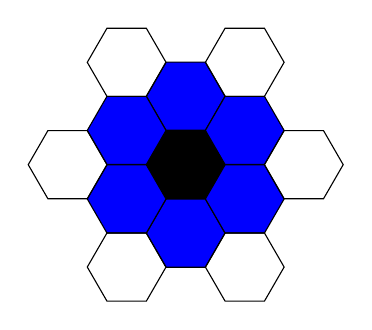
\begin{tikzpicture}
    \tikzset{
      hexagon/.style={
        regular polygon,
        regular polygon sides=6,
        minimum size=10mm,
        inner sep=0mm,
        outer sep=0mm,
        rotate=0,
        draw
      }
    }

    %Primary node
    \node[hexagon,fill=black] at (0,0) (pn) {};

    %Top node
    \node[hexagon,fill=blue] at (0,0.87) {};
    %Top right node
    \node[hexagon,fill=blue] at (0.75,0.435) {};
    %Top left node
    \node[hexagon,fill=blue] at (-0.75,0.435) {};

    %Bottom node
    \node[hexagon,fill=blue] at (0,-0.87) {};
    %Bottom right node
    \node[hexagon,fill=blue] at (0.75,-0.435) {};
    %Bottom left node
    \node[hexagon,fill=blue] at (-0.75,-0.435) {};

    %Far right node
    \node[hexagon] at (1.5,0) {};
    %Far left node
    \node[hexagon] at (-1.5,0) {};

    %Far top right node
    \node[hexagon] at (0.75,1.30) {};
    %Far top left node
    \node[hexagon] at (-0.75,1.30) {};
    %Far bottom left node
    \node[hexagon] at (-0.75,-1.30) {};
    %Far bottom right node
    \node[hexagon] at (0.75,-1.30) {};
  \end{tikzpicture}
\end{document}